% 来源：OEBPS/Text/Section0001_split_002.xhtml#sigil_toc_id_20

\BookChapter{11}
\section[第11章\q 投资营销谎言6：“目标日期基金”]{第11章\\ 投资营销谎言6：“目标日期基金”}

\begin{BookQuote}
每过一天，我对目标日期基金就愈加紧张不安。

\hfill ——约翰·博格
\end{BookQuote}

当你查看你的401(k)计划中的投资选择时，你有没有感到非常奇怪？他们怎么会弄出这样的一个投资选择名单？为什么你的配偶或者最好的朋友在同一个镇上工作，却拥有完全不同的投资选择菜单？

就像那句俗话所说的：永远跟着钱走。

\subsection{你得花钱才能玩}

在公募基金的世界里要分到一笔收入，一个常见的做法是大家都知道的，就是花钱才能参加游戏的费用。根据韬睿惠悦这个全球性的咨询公司的调查，接近90\%的401(k)计划都要求基金公司支付花钱才能参加游戏的费用，作为交换，可以把一只基金加入你的401(k)计划的基金可选菜单中。不花钱，基金就进不了门，因为根本没有机会。花钱才能参加游戏的费用，实质上是保证客户（你和我在内）只能得到有限的选择，最终只能从菜单中选择拥有一只基金，而这只基金对于经销商（即经纪人、证券公司、基金公司）来说肯定是赚钱的。换句话说，你的401(k)计划里面的投资选择，都是人家精心设计和筛选过的，好让那些销售人员、经纪人、银行理财经理、基金经理的利益最大化。如果必须花钱才能参加游戏，他们肯定会想方设法地让自己的利润最大化，以补偿他们为加入游戏多支出的成本。目标日期基金有时被称为生命周期基金，作为努力进入你个人养老金计划的投资选择的创意，它也许是最昂贵的，也是最广泛的营销。（先锋公司超低成本的目标日期基金属于例外。）

\subsection{目标日期基金偏离预定目标了吗？}

尽管是公募基金行业成长最快的品种，目标日期基金也许完全偏离了原定的目标。

那些营销广告都是这样说的：“你只要选择你要退休的年度和日期，我们就会相应配置你的投资组合（比如目标2035黄金年度基金）。你离退休的日子越近，投资组合就越保守。”我敢肯定你在自己的401(k)计划可选基金名单里看到过这样的目标日期基金。统计数据表明，你很可能会投资其中的一只目标日期基金。

这些目标日期基金到底是怎么运作的？我们来进一步做详细了解。

基金经理要决定一个“下滑路径”，这是用一个想象出来的方式来描述他们的股票仓位的调整方式：不断调降股票仓位（风险更大），不断提高债券仓位（传统上被认为风险更小），努力做到离你的退休日期越接近，你的投资组合越保守。不用说，每个基金经理可以选择自己的调降路径，其实并没有一个统一的标准。这个下滑路径让我听起来更像一个灾难性的急剧下滑。我要再说一下，这种调降路径的想法其实建立在两个特别大的前提下：

1.债券是安全的。

2.债券的波动方向与股票相反。所以，一旦股票出现下跌，你持有的债券反而会上涨，能够保护你的投资组合整体市值不会减少。

正如沃伦·巴菲特所说的，“债券应该被贴上一个风险警告标签”。因为利率上涨会让债券价格下跌，如果预测或者遇到利率上升，我们会看到债券价格暴跌（债券基金的净值也会跟着暴跌）。另外，很多独立研究表明在经济糟糕的时候，债券跟股票有很强的“相关性”。也就是说，股票和债券并不总是相反方向波动的。只要看一看2008年债券和股票一起暴跌，你就明白了。业内称之为股债双杀。

目标日期基金的市场营销术，非常有诱惑力。选择一个退休日期，你就再也不用管了。“设好，忘掉。”只要相信我们就行了，我们会照顾好你的。但是他们真的能做到吗？

\subsection{一个巨大的误解}

行为研究协会受投资咨询公司安永委托做了一个调查。结果发现，投资目标日期基金的雇员存在一些重大的误解，简直会让人惊讶得下巴都掉了：

\begin{itemize}
\item 57\%的受访者认为他们的投资在未来十年不会亏钱，但是他们根本没有事实依据来支撑这种观念。
\item 30\%的受访者认为，目标日期基金会提供有保证的投资收益率。目标日期基金没有给你任何方面的任何保证，更不用说保证投资收益率了。
\item 62\%的受访者认为，到基金到期的年份或者目标日期，他们就能够顺利退休了。不幸的是，这种错误的感觉是最惨痛的一种错觉。你设定的退休日期，只是你自己设定的退休年份目标而已。目标日期基金并不是那种能够让你达成目标的计划，它只是一种资产配置，让你越接近目标退休日期，整个资产配置组合的风险就越低。
\end{itemize}

考虑到有数万亿美元被投资在目标日期基金上，将来肯定会有相当大比例的美国投资人感到非常震惊，目标日期到了，但你根本无法实现自己的退休目标。

那么你购买目标日期基金真正买到的是什么？你只不过买了一只基金，来为你操作资产配置而已。就这么简单。你本来要从一组基金中选择资产配置，现在你买了一只基金，只用这一只基金做资产配置，就这样简单！这一只基金“全部帮你搞定”。

\subsection{抱歉，她不在这里工作了}

大学毕业之后，戴维·巴贝尔想到世界银行工作。世界银行毫无疑问是一个很有趣的工作场所，但是对于那些足够幸运、能够在那里工作的人来说，世界银行还有更大的好处，就是不用支付任何税收！真是聪明的家伙。戴维提出申请，但是世界银行的人把他拒绝了，理由是他需要拥有六类专业的研究生学位之一，才能得到这份工作。为了避免再次遭到拒绝，戴维决定得到所有这六种研究生的学位，他拿了一个经济学学士学位，一个国际金融工商管理硕士学位，一个金融哲学博士学位，一个辅修的食品与资源经济学博士学位，一个热带农业博士学位，一个拉丁美洲研究的博士学位。拿了这一堆文凭后，他再次到世界银行申请工作。结果，他们说世界银行不再鼓励雇用美国人，因为最近华盛顿削减了对世界银行的财务支持。这真是给他心头重重一击。正在不知道去向何方时，他看到加利福尼亚大学伯克利分校在报纸上刊登的招聘广告，于是他马上去信应聘。加州大学伯克利分校雇用他做教授，之后，他才发现，学校刊登广告其实只是为了遵守《平权法案》，根本没有打算让合格的候选人前来应聘。

过了几年，他转到沃顿商学院，教授很多与金融相关的课程。但他并不是一个书呆子，他写了一篇论文，探讨如何减少投资组合的风险，因此他受到了高盛公司的注意。于是，他掌管了七年高盛公司的风险管理和保险部门（与此同时，他继续在沃顿商学院担任兼职教授）。后来他终于有机会进入世界银行工作，也同时为美国财政部和联邦储备局提供咨询服务。但是当美国劳工部让他做一个反求研究，以确认目标日期基金是否真的是最佳默认退休养老金的投资选择时，他根本不知道要采取什么样的研究路径。在这个人人皆知的投资通道的另外一边是投资公司研究所（这是公募基金行业游说美国政府和国会的机构），它们“已经支付200万美元来做一项研究，其研究结果正好完全符合它们的想法。这项研究声称目标日期基金是自切片面包发明以来的最好发明”。请记住，切片面包坊出现的时候，目标日期基金仅仅是一个空泛的概念。在整个金融行业看来，它只是一丝微弱的光芒。

戴维·巴贝尔为美国劳工部做的研究，是与其他两个教授共同合作的，其中一位得到过两位诺贝尔经济学奖获得者的培训。戴维·巴贝尔把目标日期基金比作稳定价值基金。稳定价值基金超级保守，不会发生亏损，历史收益水平比货币市场基金高出2\textasciitilde{}3个百分点。按照戴维·巴贝尔的说法，那项由行业赞助的研究把目标日期基金美化得无比光鲜亮丽，但其实这种基金充满了漏洞。为了让目标日期基金看起来比稳定价值基金更美，他们虚构出来的东西比迪士尼公司的还要多。例如，他们假定股票和债券没有任何联系。大错特错！股票和债券确实在某种程度上会同步行动，在经济困难时期，它们的波动会更加相近。（股票和债券在2008年有80\%的相关性。）

戴维·巴贝尔和他的团队评估了那项由行业赞助的研究，把它拆分开来。他们从数学上分解了那项报告中的虚构性发现，准备好揭示其荒谬可笑的假定，这种假定让目标日期基金看起来非常优秀。

演示研究结论的那一天，戴维·巴贝尔准时出现，坐在桌子后面的经济学家是由美国劳工部挑选出来的评估双方研究成果的专家。这位经济学家“认为戴维·巴贝尔有一些很好的观点，需要进一步评估”。但是美国劳工部部长“已经做出了自己的决定，然后第二天就退出会议了。她甚至没有出席和戴维·巴贝尔预先安排好的会议”。巴贝尔博士听说这都是事先安排好的。基金行业已经买通了美国劳工部，得到了它需要的正式许可，给自己开具了“饱和”支票。

目标日期基金开始飞速发展，到2013年年底，41\%的401(k)计划参与人都使用了目标日期基金，它的总规模达到了万亿美元的数量级别。基金行业花钱搞的这项研究，尽管戴维·巴贝尔和他的受人尊敬的经济学家同事称其具有严重缺陷，但只花了200万美元，就换来了万亿美元的规模，这笔投资收益率还算不错。

一部2006年出台的法律为目标日期基金成为退休养老金默认的投资选择铺平了道路。雇主不再为把雇员的资金放到目标日期基金而承担责任。现在所有雇主中有超过一半的人会让雇员“自动登记”加入401(k)计划。根据富达投资集团的研究，超过96\%的大型雇主用目标日期基金作为默认的投资选择。

\subsection{潮水没有退去之前，你不会知道谁在裸泳}

想象一下，现在是2008年年初，你快要退休了，你已经辛辛苦苦地工作超过40年，拼命地赚钱养家糊口，你盼望着退休，好有更多的时间陪陪孙子、孙女们，有更多的时间去旅游，哪怕只有更多的时间休息也好。大家都说你的401(k)账户余额看起来很健康。你买的“2010年目标日期基金”业绩表现很好。你相信，由于你只有两年就要退休了，你的基金投资会非常保守。数百万美国人都有这样的感觉，结果2008年的金融危机让退休的希望彻底破灭，至少他们期望退休后享受的生活品质是肯定达不到了。图 \ref{fig:11-1} 列出了按照规模排名前20的目标日期基金，以及2008年它们让人心痛的糟糕业绩表现。请不要忘记，这些可都是2010年目标日期基金，这些基金的投资人只有两年就要退休了。请注意，这些基金选择投资股票的仓位比例是多么高，尽管投资者原本以为这些基金接近“最后阶段”，因此应该是最保守的。公平地讲，即使你就要退休了，你也必须在股票上有一定的仓位，但是与此同时，这种损失可能会彻底毁掉你的退休计划，至少会拖延你的退休计划。

\begin{figure}[htbp]
\centering
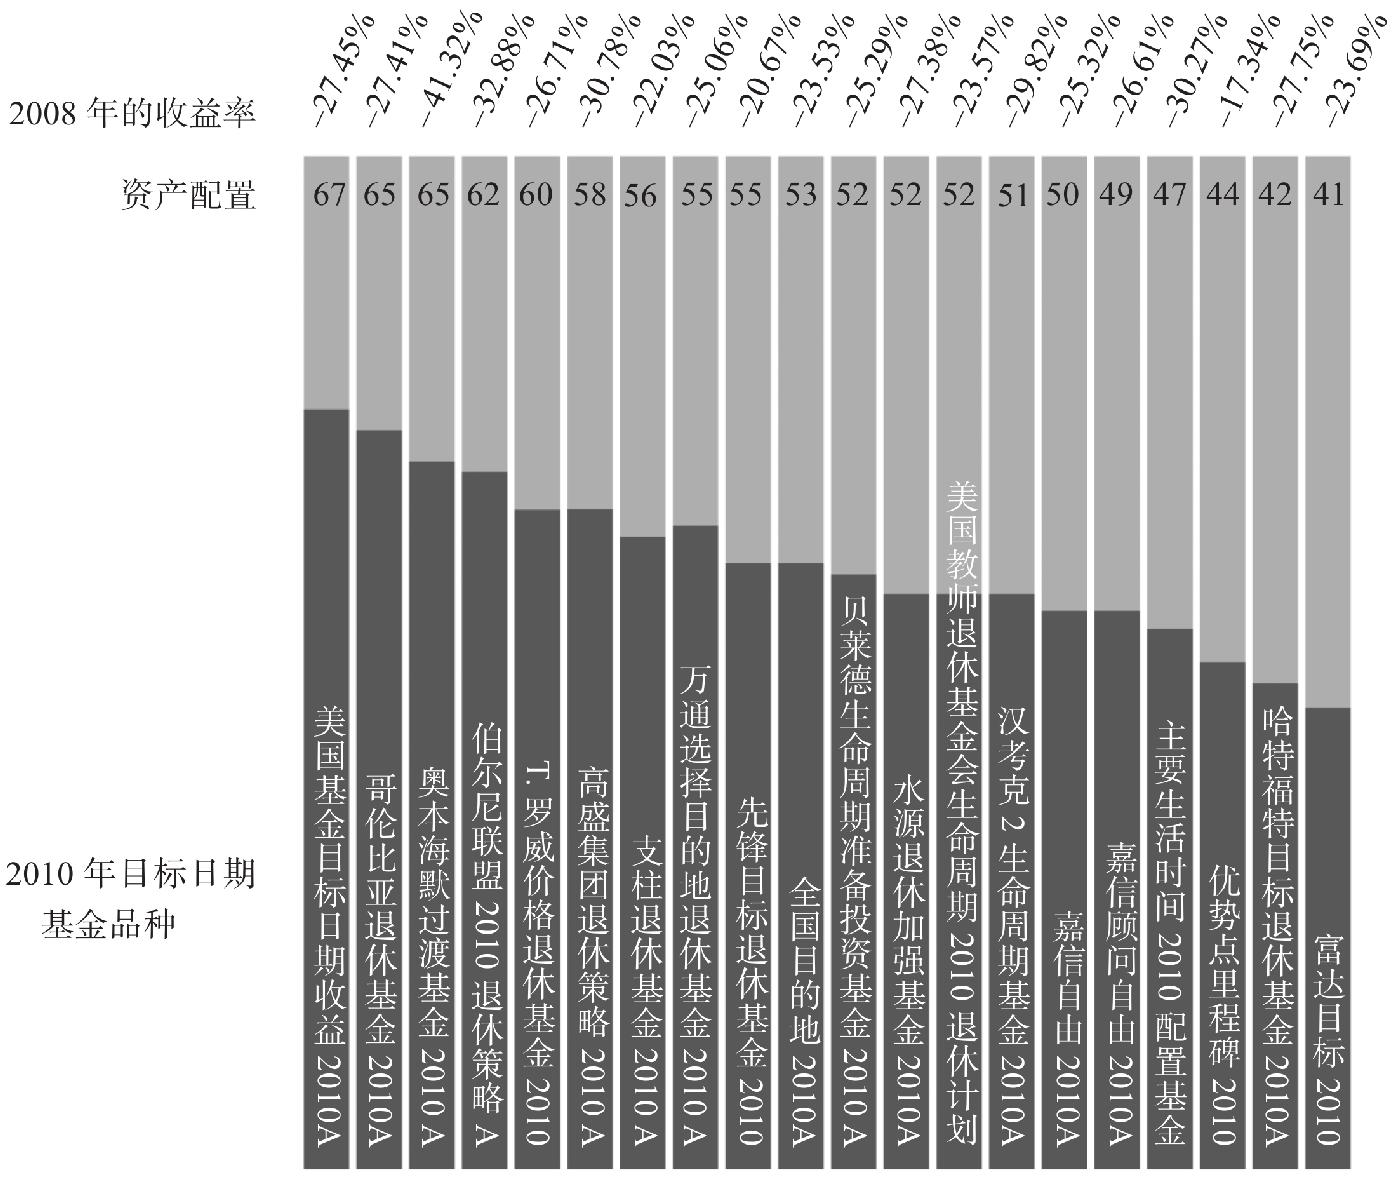
\includegraphics[width=0.84\linewidth,keepaspectratio]{image/11-1.jpg}
\caption{}\label{fig:11-1}
\par\smallskip{\footnotesize 资料来源：晨星评级机构\par}
\end{figure}

\subsection{两害相权取其轻}

我采访了很多退休研究领域的顶尖的学术专家，结果令我非常吃惊，他们都十分支持目标日期基金。

稍等一下。怎么会是这样？

我给他们分享了大部分你刚才读过的内容，尽管他们并不同意目标日期基金确实存在上述的那些问题，但是他们同时指出在目标日期基金出现之前，其实人们拥有很多选择，可以完全按照自己的意愿进行资产配置。结果这种安排导致出现更多困惑，坦白地讲，这也导致出现很多非常糟糕的投资决策。统计数据当然完全支持他们的观点。

我就这个问题采访了杰弗里·布朗，他肯定拥有美国最聪明的脑袋。他解释道：“如果你回到这些东西（目标日期基金）出现之前，你会看到我们很多人都是投资自己雇主公司的股票。他们的投资过度集中在自己雇主公司的股票上。”他的这些话让我想起了安然公司，很多安然公司的雇员都把自己的养老金百分之百地投资在了安然股票上，可一夜之间这些养老金全都没了。

当人们面对15项不同的公募基金进行选择时，他们就会把钱平均分配（15只基金，每只投资1/15的资金），这并不是一个好的投资策略。他们一遇到股市下跌就会紧张害怕（或者股市一跌就会卖出），然后就一直守着现金，好几年不敢投资股票。你用一部分来持有现金，并不是糟糕的资产配置，但是在401(k)计划里，你要为这个计划本身支付费用，你一直持有现金，就会承担双重损失：一是照样要付计划管理费，二是要承担通货膨胀带来的现金贬值损失。简言之，我可以理解布朗博士的看法。

你觉得目标日期基金的概念有吸引力，但布朗博士推荐低成本指数基金，就像先锋公司提供的指数基金那样。如果有人只有最低投资金额，情况非常简单，花钱找个投资顾问完全是多余的，那么这些人选择目标日期基金可能是个不错的投资途径。但是如果你不想使用目标日期基金，并且有途径能够得到一个低成本指数基金的名单，那么你可以从中选择投资，运用本书后面讲解的资产配置模式。资产配置是指把你的钱放在哪里和如何划分投资比例，这是成为一个成功投资者最重要的技巧。我们后面会跟大师学习，你会发现其实资产配置并不是那么复杂难懂。低成本目标日期基金对于一般投资者来说也许非常不错了，但是你并非一般的投资者，因为你正在读本书。

此外，很多人认为并没有很多替代目标日期基金的选择，但是在第五部分，你会学到一种特别的资产配置方案，由对冲基金大师瑞·达利欧设计。它创造出了非常出色的收益，而且只有极小的下跌风险。一个分析师团队回测了这个投资组合，在过去75年里，最糟糕的亏损只有3.93\%。相反，MarketWatch网站（一个财经网站）上报道：“最保守的目标日期基金（为产生退休收入而设计）在2008年的平均跌幅为17\%，最危险的目标日期基金（为2055年的退休者设计）在2008年的平均跌幅为39.8\%，这个数字非常惊人。这是伊博森协会最近一份研究报告的统计数据。”

\subsection{又干掉了一个谎言}

我们又揭露了一个投资营销谎言。我想，到现在为止，你开始明白无知并不是福气，在金融世界里，无知是痛苦，是贫穷。前面几章让你获得的知识会成为你投资需要的动力，让你能够说出来：“我再也不要让人占便宜了！”

很快，我们就会开始探索令人激动的投资机会、投资策略、投资工具，帮助你创造财务自由。但是在此之前，我们还有两个投资营销谎言需要识破。
